% Created 2021-02-08 pon 15:45
% Intended LaTeX compiler: pdflatex
\documentclass[11pt]{article}
\usepackage[utf8]{inputenc}
\usepackage[T1]{fontenc}
\usepackage{graphicx}
\usepackage{grffile}
\usepackage{longtable}
\usepackage{wrapfig}
\usepackage{rotating}
\usepackage{float}
\usepackage[normalem]{ulem}
\usepackage{amsmath}
\usepackage{textcomp}
\usepackage{amssymb}
\usepackage{capt-of}
\usepackage{hyperref}

\usepackage[nottoc]{tocbibind}
\author{Łukasz Piotrak}
\date{\today}
\title{An analysis of dimensionality reduction and music information retrieval techniques for the visual representation of large audio datasets.}
\hypersetup{
 pdfauthor={Łukasz Piotrak},
 pdftitle={An analysis of dimensionality reduction and music information retrieval techniques for the visual representation of large audio datasets.},
 pdfkeywords={},
 pdfsubject={},
 pdfcreator={Emacs 27.1 (Org mode 9.4)}, 
 pdflang={English}}
\begin{document}

\maketitle
\tableofcontents

\begin{abstract}
Abstract goes here
\end{abstract}

\section{Introduction}
\label{sec:org6dce8a9}
\subsection{Background \& Motivation}
\label{sec:orge77a0b6}
The current paradigm for the storage and organization of audio files is that of the classic directory tree. This results in an attribute ontology; files are grouped together into classes (usually by directory name) i.e. ``Drums'', ``Vocals'' and assigned a range of attributes by means of file name or tags. This approach is limited, e.g. the file might be labeled incorrectly or the labels might not addequately describe the sound. Moreover, many properties inherrent to the files are hard to represent e.g. two audio samples might be in separate branches of the taxonomy but be perceptually similar. However, as shown by projects such as The Infinite Drum Machine by Google Creative Lab, collections of sounds can be explored more naturally with the help of dimensionality reduction techniques.

Advances in this area have enabled the intuitive representation of high-dimensional data. The dimension count of a Dataset can be reduced arbitrarily while still preserving information about its intrinsic properties. Commonly, this approach is used to plot Datapoints as clouds in 2d or 3d space, allowing for a depiction of the data which can be naturally grasped by the human mind.

As with many kinds of information, audio data in its raw form is unfit for such processing. An intermediate representation must to be constructed if any insights are to be gleaned from the data. In order to obtain a representations of audio signals useful to a human observer, a selection of features have to be extracted, which might correspond to certain aspects of the human perception of sound. These can then be used as inputs to produce a visualization by means of dimensionality reduction.

The goal of this paper is to provide an evaluation of both feature extraction and dimensionality reduction techniques, apply them to a large set of audio data and determine which combination of the two gives an optimal visual representaion.

\subsection{Related Work}
\label{sec:org42eee01}
\subsubsection{The infinite drum machine}
\label{sec:org4401227}
\subsubsection{Klustr}
\label{sec:org02aa748}
\subsubsection{Other Commercial products}
\label{sec:orgc78ac43}
\section{Background}
\label{sec:org4d1b31d}
\subsection{Machine learning and audio}
\label{sec:orgafd5aa0}
\subsection{Music information retreival}
\label{sec:orge32af72}
\subsubsection{Signal processing}
\label{sec:org19fe369}
\begin{enumerate}
\item The fourier transform
\label{sec:org8e1fd90}
\item Sampling and the dirac delta function
\label{sec:orgd9ae2f1}
\item The fast fourier transform
\label{sec:org49e433d}
\item Signal processing and limitations
\label{sec:orgcde52dd}
\end{enumerate}
\subsubsection{Pre processing steps}
\label{sec:orgdd5f8ff}
\begin{enumerate}
\item Down mixing
\label{sec:org38fd0e8}
\item Normalization
\label{sec:orgda013eb}
\end{enumerate}
\subsubsection{Short-term Fourier Transform (stft)}
\label{sec:org5ad94c1}
The Short-term Fourier Transform is a representation of a signal obtained by taking the Fourier transform of short, overlapping segments of time. The method used to obtain the stft is relatively straightforward:
First, the signal is divided into shorter, equal-length segments over time using a window function. Multiple window functions could be used for this step, however a

Next, the DFT is computed for each segment. We can thus observe how the frequency content of the signal changes as we progress through time.
\subsubsection{MFCC}
\label{sec:org657745a}
\subsubsection{MIR metrics}
\label{sec:org59595af}
\begin{enumerate}
\item spectral centroid
\label{sec:org722ed3e}
\item spectral rollof
\label{sec:org8ba1512}
\item spectral bandwidth
\label{sec:org9dcacf6}
\item spectral crest
\label{sec:org25d762a}
\item specral flux
\label{sec:org8d3ce71}
\item spectral flatness
\label{sec:org06c8a6d}
\item RMS
\label{sec:orgb1f5108}
\item zero-crossing rate
\label{sec:org7b27629}
\end{enumerate}
\subsection{Dimensionality reduction}
\label{sec:orgb502774}
\subsubsection{PCA}
\label{sec:org93f3c9b}
\subsubsection{t-sne}
\label{sec:orgadaa38f}
\subsubsection{umap}
\label{sec:org6a758a8}
\subsection{Evaluation metrics}
\label{sec:org078e27c}
\subsubsection{Silhoutte score}
\label{sec:org8d91088}

The Silhouette Coefficient for a sample \(i\) is given by the equation
\[s(i) = \frac{a(i) - b(i)}{\max{a(i), b(i)}} \]
Where \(a\) is the mean distance between a sample \(i \in C_{i}\) and all other points in the same cluster \(C_{i}\). This gives us how close a point is to the corresponding cluster. It is given by the equation:
\[ a(i) = \frac{1}{|C_{i}| - 1} \sum_{j \in C_{i}, i \neq j}{d(i,j)}\]
where \(d(i,j)\) is the distance between points \(i\) and \(j\).

\(b\) is the mean distance between a sample \(i \in C_{i}\) and all other points in the next nearest cluster \(C_{k}\). Given by:
\[ b(i) = \min_{k \neq i}{\frac{1}{|C_{k}|} \sum_{j \in C_{k}}{d(i,j)}} \]

The final Silhouette score for a clustering is the mean Silhouette Coefficient over all the datapoints:
\[ \frac{1}{|I|}\sum_{i \in I}{s(i)} \]
Where \(I\) is the set of all datapoints. The final value is in the range \([-1, 1]\) with values closer to -1 indicating incorrect clustering and values closer to +1 indicating highly dense clustering. Scores around zero indicate overlapping clusters. The score is generally higher for convex well-sperated and dense clusters.

\subsubsection{Roundness}
\label{sec:org7b61201}

The overall roundness of the plot is calculated by using the method proposed by Polsby \& Popper \cite{popper}:
\[PP(D) = \frac{4 \pi A(D)}{P(D)^{2}} \]
where \(D\) is the convex hull of all points of the plot, \(P(D)\) is the circumference and \(A(D)\) the area.
\subsubsection{Overlap of cluster convex hulls}
\label{sec:org274a5d2}

The measure of overlap of the convex hulls of each class. I calculate this by taking the ratio of the area of the unary union of convex hulls of each class to the sum of areas of the convex hulls of each class:
\[ O = \frac{A(U)}{\sum_{c \in C}A(H_{c})} \]
Where \(A(U)\) is the unary union of all convex hulls, \(A(H_{c})\) is the area of the Hull for class c and \(C\) is the set of all classes.
\subsubsection{Ripleys K function}
\label{sec:org533d625}

Ripley's K function is sum of the number of points N within a distance r of a selected point p, per area \(\lambda\) surrounding p. This  value is normalized by the total points:
\[K(r) = \frac{\sum_{i=1}^{n}N_{p_{i}}(r)}{n \lambda}\]
It may be interpreted as a meassure of deviation of a given distribution from the random Poisson distribution. In essence, this let's us measure the homogeneity of the spatial density of the data points. The expected value of \(K(r)\) for a random distribution is \(\pi r^{2}\). If the output value deviates from this value, this indicates clustering or dispersion in the data. The K-function may be normalized so that the expected value is r:
\[L(r) = \sqrt[]{K(r)/\pi}\]
Further normalization gives an expected value of 0, called the H-function:
\[H(r) = L(r) - r\]
Now, a positive value of \(H(r)\) indicates that the data is clustered at the scale of r. If the value is negative, the data is dispersed.

\section{Experiment design and overview}
\label{sec:orga220b5b}
\subsection{Dataset}
\label{sec:orgac308b8}

I used the Medley-Solos-db dataset assembled by Lostanlen et al. \cite{medley}. Downloaded through the mirdata python library \cite{bittner_fuentes_2019}. The dataset consists of 21572 mono WAV files sampled at 44.1 kHz at a bit depth of 32. Every audio clip has a duration of 2972 milliseconds. The data is split into 3 subsets: training, validation and test. Each sample belongs to one instrument category among a taxonomy of 8. Each instrument class was given a distinct color for easier recognition on the plots as seen in \ref{fig:8-plots}.
\begin{figure}[h]
\centering
\includegraphics[width=.9\linewidth]{./Figures/8_samples.png}
\caption{\label{fig:8-plots}Selected sample belonging to each of the instrument classes. Each consists of 65,536 32-bit floating point numbers.}
\
\end{figure}

\subsection{The processing pipeline}
\label{sec:org82c3cb3}

To produce a 2d scatter plot of the dataset, the original audio files, each an array of 65,536 floating-point numbers, has to be reduced to 2 values.
The process can be thought of as having 4 distinct steps:
\begin{enumerate}
\item Preprocessing.

The audio files are ingested in a format which is easy to run calculations on. In this case a numpy ndarray.
\item Feature Extraction.

Some characteristics of the sound are extracted using a selection of algorithms and mathematical tools. These are then used as an intermediate representation of the sound for further processing.
\item Feature manipulation

Some of the features had to be further modified after extraction. The operations included reshaping feature matrices and aggregation.
\item Dimensionality Reduction.

After selecting a set of features to serve as a representation of the original files an algorithm is applied to reduce them to two dimensions.
\end{enumerate}
Once the plots have been generated, the one which most closely fits the defined criteria must be chosen. As such, an extra, fourth step in which plots are evaluated must be added. Each of these steps will be described in greater detail in the next section.

\subsection{Preprocessing}
\label{sec:org1f10704}

The data is ingested using the Librosa python library \cite{librosa} used for music and audio analysis. The ``librosa.load'' method was used to convert the WAV files to a float32 numpy ndarray.

\begin{figure}[h!]
\centering
\includegraphics[width=.7\textwidth]{./Figures/original_sample.png}
\caption{\label{fig:example-fig}A sample from the clarinet class}
\end{figure}

After loading the samples, the amplitudes were normalized to be in the range \([-1, 1]\) by dividing by the max amplitude value for the sample. The data loaded in such a way was stored in a hdf5 file.

\subsection{Feature Extraction}
\label{sec:org8d85bd5}

Finding a compact representation of phenomena is crucial for machine learning processess, including dimensionality reduction. To produce a meaningful representation of the raw data, useful to machines as well as humans, the step of extracting features is required. It can be even thought of as a preliminary dimensionality reduction technique as a raw signal consisting of many thousands of values to just a handful, which, with luck, provide an adequate representation of useful characteristics, innate to the signal. Most of the feature extraction steps were calculated using the implementations found in the librosa library.


\subsubsection{STFT}
\label{sec:org0c9e9c5}

The Short-time Fourer Transform is a basic representation in signal processing, which captures the change in frequency content over time.
To extract the stft, I used the librosa implentation. I decided to take the STFT over 32 windows in both the time and frequency domains, finally giving a 32x32 matrix:

\begin{figure}[H]
\centering
\includegraphics[width=.7\linewidth]{./Figures/stft.png}
\caption{STFT of the sample in figure \ref{fig:example-fig}}
\end{figure}

\subsubsection{MFCC}
\label{sec:org70aa9fd}

The Mel-Frequency Cepstral Coefficients are a heavily used in both speech recognition and MIR. \cite{medium,klustr,Racharla_2020,article}
I used the librosa implementation to calculate the mfcc's. I decided to go with a Cepstral Coefficient count of 20 and hop length of 256, resulting in a feature size of 20x257:

\begin{figure}[H]
\centering
\includegraphics[width=.7\linewidth]{./Figures/mfcc.png}
\caption{MFCC of the sample in figure \ref{fig:example-fig}}
\end{figure}

\subsubsection{MIR Metrics}
\label{sec:orgb3249b0}

A number of metrics from the field of audio analysis has also found to be useful when extracting timbre information from audio signals \cite{article,klustr}. In my case these will include:

\begin{itemize}
\item Root mean square
\end{itemize}

\begin{itemize}
\item Spectral Centroid
\end{itemize}

\begin{itemize}
\item Spectral Crest
\end{itemize}

\begin{itemize}
\item Spectral Flux
\end{itemize}

\begin{itemize}
\item Spectral Roll
\end{itemize}

\begin{itemize}
\item Zero crossing Rate
\end{itemize}

\begin{figure}[H]
\centering
\includegraphics[width=.7\linewidth]{./Figures/mir_features.png}
\caption{Graphs of MIR features for the sample in figure \ref{fig:example-fig}}
\end{figure}

\subsection{Feature Manipulation}
\label{sec:org694b75f}

Many of the features are of different shapes and sizes. Since the matrix passed to the dimensionality reduction algorithm must be rectangular (i.e. a vector for each sample) a way must be found to force the features into a 1-d vector of values. I have used two approaches.

\begin{itemize}
\item Flattening

If the feature matrix is 2 dimensional, we can simply concatenate consecutive rows into one feature vector transforming a \((k,n)\) shape matrix to an array of length \(k \times n\). The raw STFT and MFCC feature matrices must be flattened in this way to be used in the further steps of dimensionality reduction.

\item Aggregation over selected axis

Another approach to reducing feature dimensions is that of aggregation. We can calculate an aggregate value over a particular axis, in essence reducing the dimensionality of the matrix by this axis. We can then treat the reduced matrix as any other feature vector. As suggested by Dupont et al. \cite{Dupont_2013} and Fedden \cite{medium}, I chose three aggregation functions: the average, standard deviation, and the mean of the difference between consecutive values in the vector.

In my case this procedure was applied to the following features:
\begin{itemize}
\item raw stft, reducing size from 32x32 -> 32x1.
\item raw mfcc, reducing size from 20x257 -> 20x1.
\end{itemize}
\end{itemize}

\subsection{Dimensionality Reduction}
\label{sec:orgfde1e30}

The last step in the pipeline is the final dimension reduction of the final collection of features to just 2 values. 4 different algorithms were used in this step:
\begin{itemize}
\item Principal Component Analysis

The basic, tried-and-tested dimensionality reduction method. This method doesn't accept any additional parameters except the number of Principal Componenets to output. As such, for each collection of features we obtain 1 plot.
\item T-stochastic neighbour embedding

What has come to be a widespead technique in the field of machine learning for it's ability to create useful 2d maps of data. Used by McDonal et al.  and Hantrakul et al. to create visualizations of audio data. T-sne's uses extend far beyond just audio data, however. It is commonly used in the field of single-cell genomics to visualize human genetic data \cite{doi:10.1142/S0219720017500172} and is able to seperate samples from different continents and even reflects some local, sub-continental patterns.

3 parameters influence the visualization in a significant way:
\begin{itemize}
\item Perplexity, which can be interpreted as how much attention the algorithm should give to local or global structure. In the original article van der Maaten \& Hinton suggested that perplexity values should generally fall in the range 5-50. In my case, smaller values tend to result in plots with less dense clusters with higher values giving more well-seperated clusters. I chose the values [5, 10, 20, 40, 60] as parameters for the t-sne plots.
\item The learning rate. Usually falls in the range [10-10000]. I however determined that values higher than 1000 seemed to lose global structure. I chose the values [20, 50, 100, 200, 300]
\item Iterations. I decided to go with a constant value of 3000. After heuristic tests I determined that the plots seemed to be stable for this dataset.
\end{itemize}

\item Uniform Manifold Approximation and Projection

A relatively new dimensionality method. It is very effective at preserving both the local and global structure of the original data in it's projections. Similarly to t-sne it is also based on manifold learning. The important hyperparameters are:
\begin{itemize}
\item number of neighbours
This parameter controls the number of approximate nearest neghbors to use to construct the initial high dimensional graph. Low values tend to focus on the fine, local structure. Higher values put an emphasis on the wider structure since they take into account a larger number of neighbour points. I chose values [5, 10, 15, 30, 50, 100, 200]

\item minimum distance is the value used by the algorithm to determine what the minimum distance points on the embedding can be from each other. I chose to sweep throught the whole range: [0.0, 0.001, 0.01, 0.1, 0.5, 0.75, 0.99]
\end{itemize}
\end{itemize}

\begin{figure}
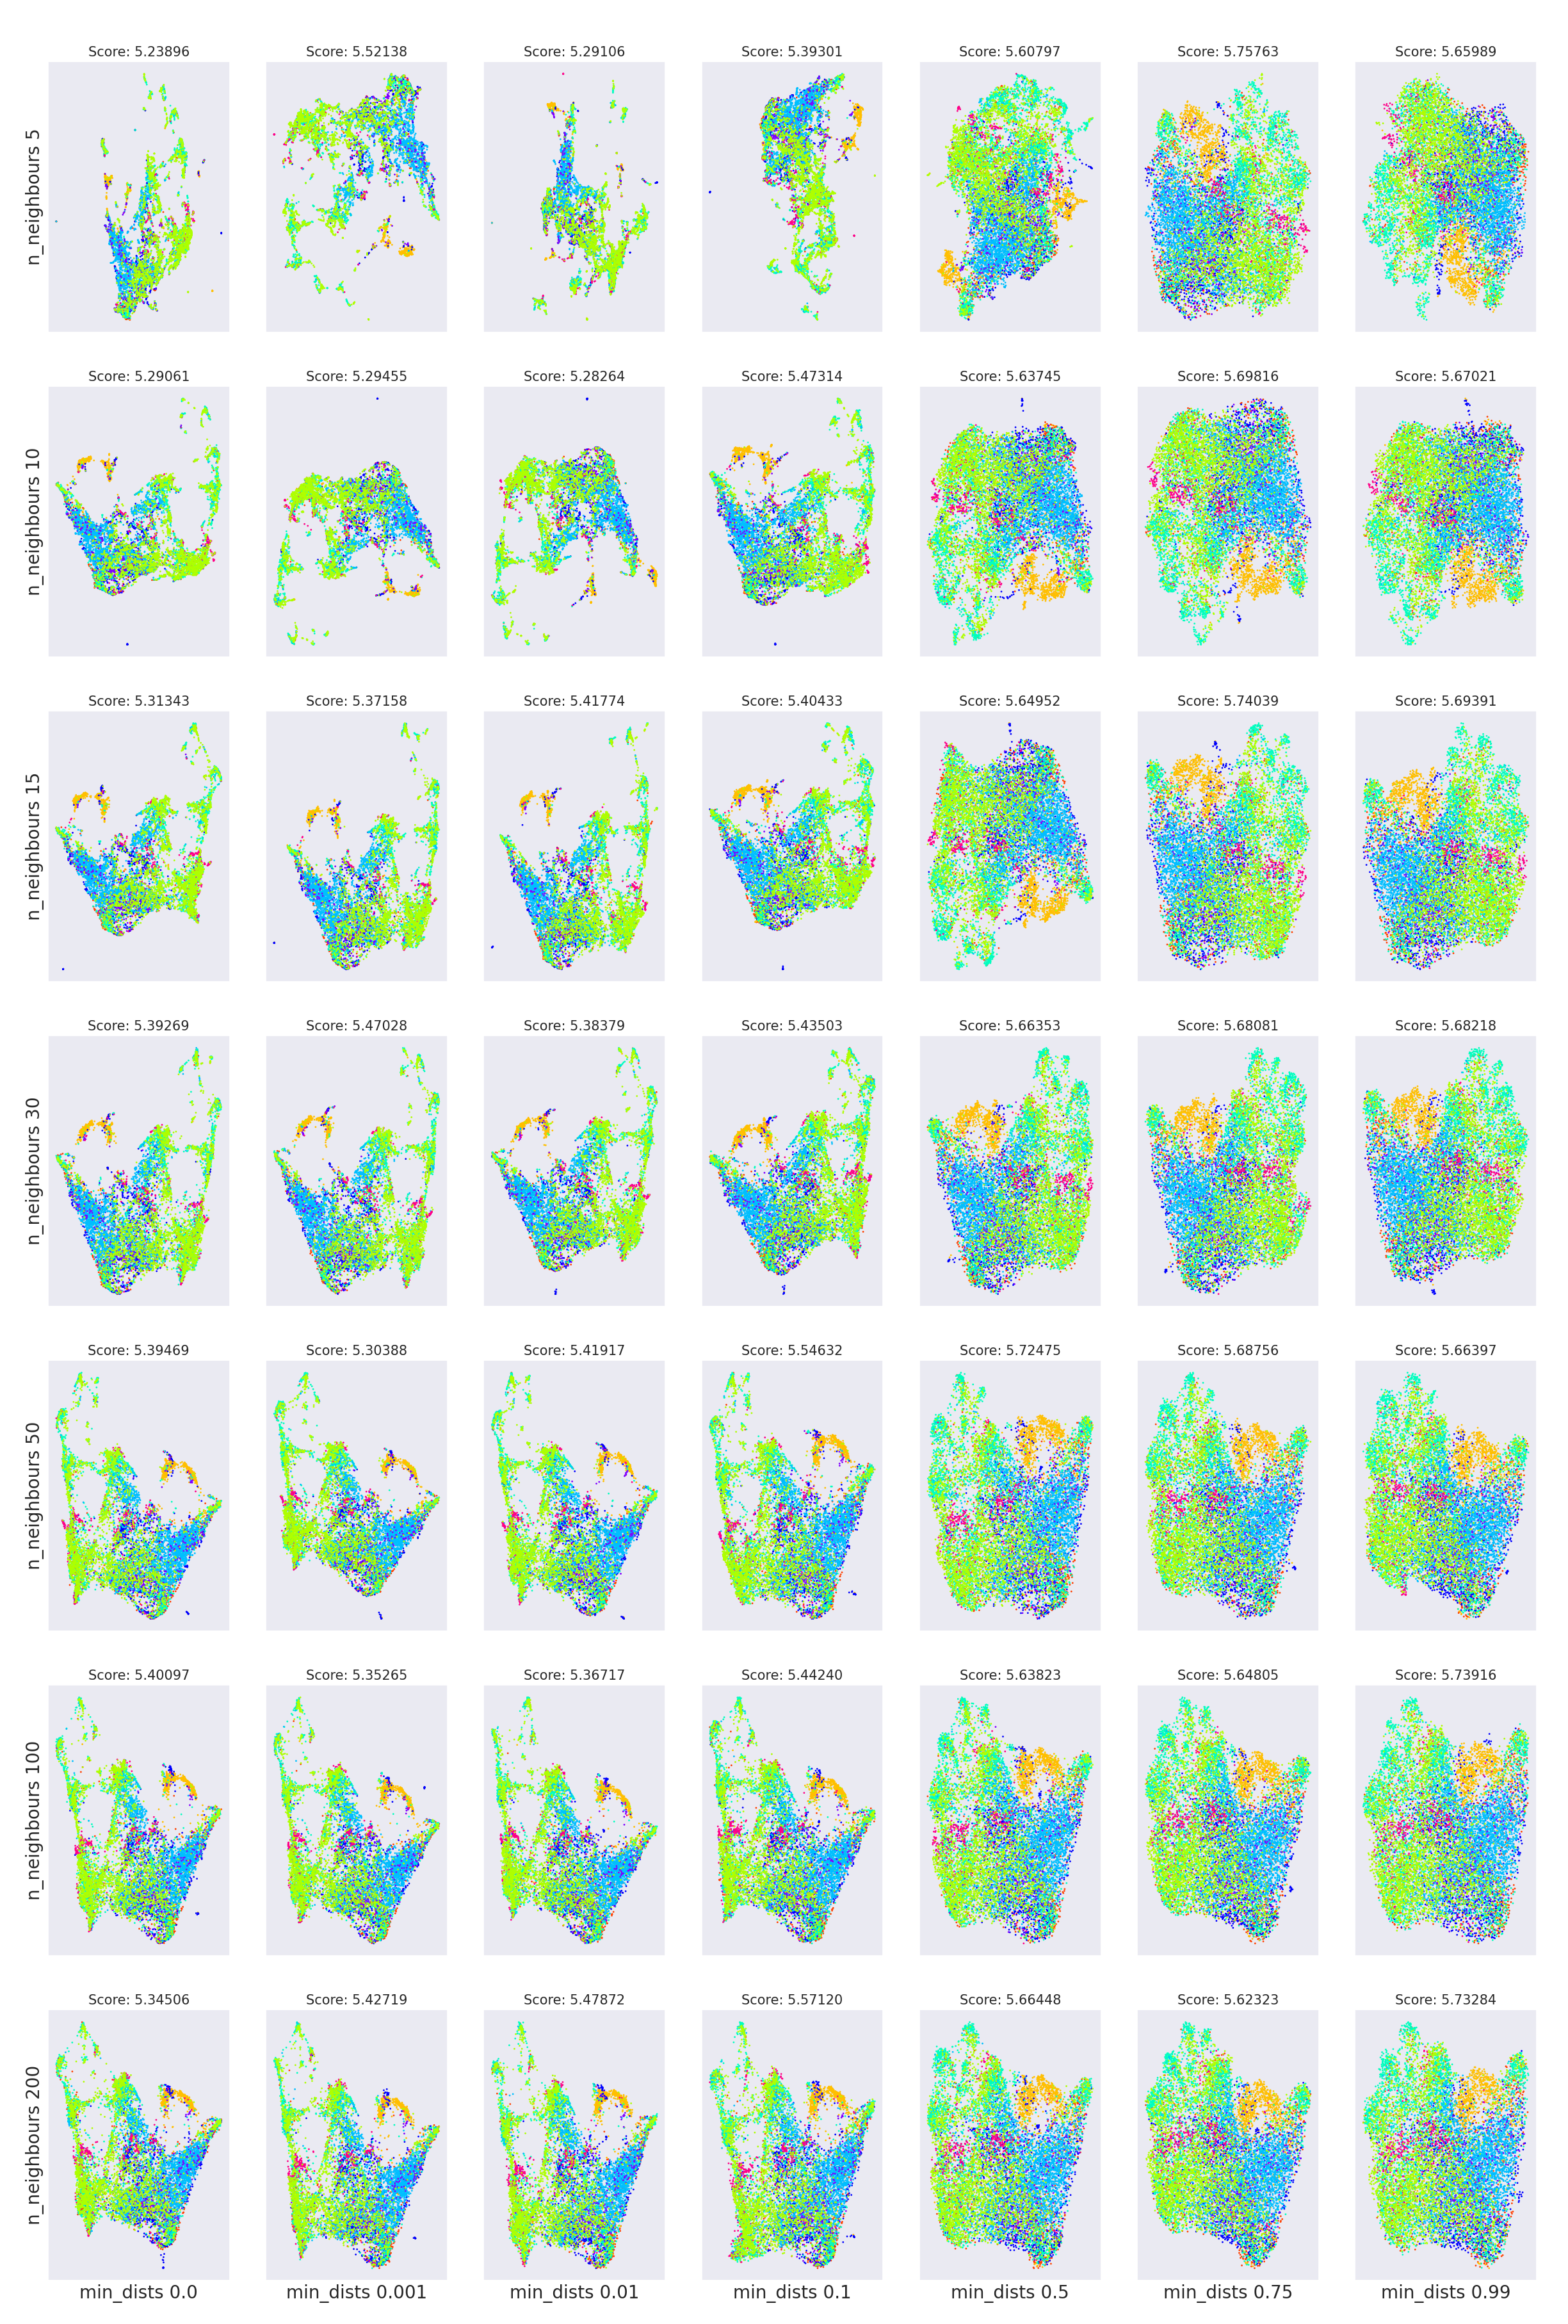
\includegraphics[width=\textwidth,height=0.75\textheight]{./Figures/umap_stft_gridsearch.png}
\caption{A Umap grid search over stft.\\ It is clear to see that lower values of hyperparameters (top left) give more densely clustered plots with a focus on the local structure, while higher values (bottom right) are more distributed and focus more on global relationships.}
\end{figure}




Since the objective is to make a round and homogenously dispersed plot, while still keeping the clusters seperate, I suspect that values, which strike a balance between being globally spread out and having enough detailed local structure to seperate the clusters will be evaluated as teh best.

\subsection{Scoring the plots}
\label{sec:org007743d}

The experiment was designed with a particular goal in mind - generating plots from the original audio data which would enable an intuitive grasp of the dataset. In order to achieve this, I define several metrics for evaluating the plots:
\begin{itemize}
\item How well the embedding reflects the inherrent relationships between datapoints. This is measured by the Silhouette score with the class labels corresponding to cluster labels. Also, the overlap of the convex hulls of classes is an indicator of this quality.
\item Readability and ease-of-navigation of the plot. In order for the plot to be readable, points should be as evenly distributed as possible, avoiding clumps, which might be hard to navigate. Ripley's function is an indicator of homogeneity of the density distribution of points on the plot. I figured, that a regular, uniform shape of the plot would increase readability, as such metric of readability is given by the Polsby-Popper method for measuring the roundness of the convex hull of the plot.
\end{itemize}
Each plot produced is scored using these metrics. Since each of these metrics had a different range of values, to compute a final score for the plot, each metric was normalized to the range \([0, 1]\). The final score for plot \(p \in P\) is a weighted sum of all the normalized individual metrics given by:
\[T(p) = 2silhouette(p) + 2ripley(p) + overlap(p) + roundness(p) \]
Where:
\begin{itemize}
\item \(silhouette(p)\) is the normalized Silhouette score. Because the silhouette metric is in the range \([-1, 1]\) the value must be shifted to be in range \([0, 1]\): \(s(p) + 1\). Where \(s(p)\) is the Silhouette score for the plot. The shifted silhouette score is then normalized relative to the max silhouette score, finally giving:
\[silhouette(p) = \frac{s(p) + 1}{\max\{s(p) | p \in P\}}\]
\item \(ripley(p)\) is a metric based on the Ripley H-function. First, the average Ripley H-function is taken for plot \(p\) for radii in the set: \(R = (0.05, 0.1, 0.25, 0.5)\) \(\sum_{r \in R} H_{p}(r)\) Since the H-function can assume values both negative and positive, I decided to take the absolute value. This causes a loss of information, since negative values indicate dispersion and positive ones indicate clustering. However, this distinction is not important for the purposes of the experiment. The only information important to us is how much the plot deviates from being uniformly dense. Since we want values close to 1 to indicate a better score I take the inverse, giving:
\[H(p) = abs(\frac{\sum_{r \in R} H_{p}(r)}{|R|})^{-1}\]
With \(H_{p}(r)\) being Ripley's H-function for plot \(p\) taken for radius \(r\). Finally, the value is normalized relative to the max value for all plots.
\[ ripley(p) = \frac{H(p)}{ \max \{ H(p)| p \in P \}} \]
\item \(overlap(p)\) is the ratio of overlap of convex hulls for the clusters to the area of the whole plot. Normalized relative to the max value for all plots:
\[ overlap(p) = \frac{O(p)}{ \max \{ O(p)| p \in P \}} \  \]
\item \(roundness(p)\) is calculated using the Polsby-Popper method. Also normalized relative to the max value for all plots:
\[ roundness(p) = \frac{PP(p)}{ \max \{ PP(p)| p \in P \}} \  \]
\end{itemize}

\section{Experiment Evaluation}
\label{sec:org8d9a4f0}


Results
\label{sec:org5ce221c}
\subsection{What could be improved}
\label{sec:org1054556}
\subsection{limitations}
\label{sec:org1e550a7}
\subsection{suggestions for future work}
\label{sec:org8e8f855}
\subsection{Conclusion}
\label{sec:orgf2b4e9e}

\bibliography{Bibliography}
\bibliographystyle{plain}
\end{document}
